\section{Section 3}

\begin{frame}{Examples}
    \begin{exampleblock}{Numbered Equation}
        \begin{equation} % Add * to remove numbering
            J(\theta) = \mathbb{E}_{\pi_\theta}[G_t] = \sum_{s\in\mathcal{S}} d^\pi (s)V^\pi(s)=\sum_{s\in\mathcal{S}} d^\pi(s)\sum_{a\in\mathcal{A}}\pi_\theta(a|s)Q^\pi(s,a)
        \end{equation}
    \end{exampleblock}
    \begin{exampleblock}{Multi-line Equation\footnote{This is a footnote}}
        % Use & to separate
        \begin{align}
            Q_\mathrm{target}&=r+\gamma Q^\pi(s^\prime, \pi_\theta(s^\prime)+\epsilon)\\
            \epsilon&\sim\mathrm{clip}(\mathcal{N}(0, \sigma), -c, c)\nonumber
        \end{align}
    \end{exampleblock}
\end{frame}

\begin{frame}
    \begin{exampleblock}{Numbered Multi-line Equation}
        % Taken from Mathmode.tex
        \begin{multline}
            A=\lim_{n\rightarrow\infty}\Delta x\left(a^{2}+\left(a^{2}+2a\Delta x+\left(\Delta x\right)^{2}\right)\right.\label{eq:reset}\\
            +\left(a^{2}+2\cdot2a\Delta x+2^{2}\left(\Delta x\right)^{2}\right)\\
            +\left(a^{2}+2\cdot3a\Delta x+3^{2}\left(\Delta x\right)^{2}\right)\\
            +\ldots\\
            \left.+\left(a^{2}+2\cdot(n-1)a\Delta x+(n-1)^{2}\left(\Delta x\right)^{2}\right)\right)\\
            =\frac{1}{3}\left(b^{3}-a^{3}\right)
        \end{multline}
    \end{exampleblock}
\end{frame}

\begin{frame}{Graph and Columns}
    % From thuthesis user guide.
    \begin{minipage}[c]{0.3\linewidth}
        \psset{unit=0.8cm}
        \begin{pspicture}(-1.75,-3)(3.25,4)
            \psline[linewidth=0.25pt](0,0)(0,4)
            \rput[tl]{0}(0.2,2){$\vec e_z$}
            \rput[tr]{0}(-0.9,1.4){$\vec e$}
            \rput[tl]{0}(2.8,-1.1){$\vec C_{ptm{ext}}$}
            \rput[br]{0}(-0.3,2.1){$\theta$}
            \rput{25}(0,0){%
            \psframe[fillstyle=solid,fillcolor=lightgray,linewidth=.8pt](-0.1,-3.2)(0.1,0)}
            \rput{25}(0,0){%
            \psellipse[fillstyle=solid,fillcolor=yellow,linewidth=3pt](0,0)(1.5,0.5)}
            \rput{25}(0,0){%
            \psframe[fillstyle=solid,fillcolor=lightgray,linewidth=.8pt](-0.1,0)(0.1,3.2)}
            \rput{25}(0,0){\psline[linecolor=red,linewidth=1.5pt]{->}(0,0)(0.,2)}
%           \psRotation{0}(0,3.5){$\dot\phi$}
%           \psRotation{25}(-1.2,2.6){$\dot\psi$}
            \psline[linecolor=red,linewidth=1.25pt]{->}(0,0)(0,2)
            \psline[linecolor=red,linewidth=1.25pt]{->}(0,0)(3,-1)
            \psline[linecolor=red,linewidth=1.25pt]{->}(0,0)(2.85,-0.95)
            \psarc{->}{2.1}{90}{112.5}
            \rput[bl](.1,.01){C}
        \end{pspicture}
    \end{minipage}\hspace{1cm}
    \begin{minipage}{0.5\linewidth}
        \medskip
        %\hspace{2cm}
        \begin{figure}[h]
            \centering
            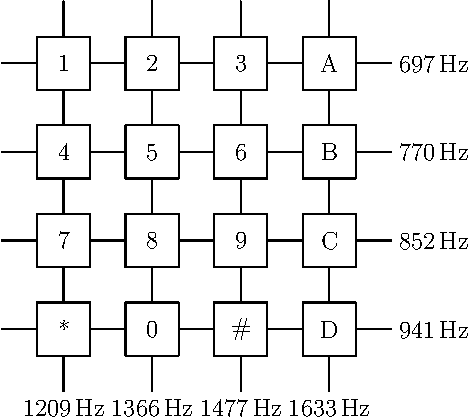
\includegraphics[height=.4\textheight]{images/dtmf.pdf}
        \end{figure}
    \end{minipage}
\end{frame}

\begin{frame}[fragile]{Common \LaTeX{} Commands}
    \begin{exampleblock}{Commands}
        \centering
        \footnotesize
        \begin{tabular}{llll}
            \cmd{chapter} & \cmd{section} & \cmd{subsection} & \cmd{paragraph} \\
            Chapter & Section & Subsection & Paragraph \\\hline
            \cmd{centering} & \cmd{emph} & \cmd{verb} & \cmd{url} \\
            Centering & Emphasis & Verbatim & URL \\\hline
            \cmd{footnote} & \cmd{item} & \cmd{caption} & \cmd{includegraphics} \\
            Footnote & Item & Caption & Graphics \\\hline
            \cmd{label} & \cmd{cite} & \cmd{ref} \\
            Label & Cite & Reference\\\hline
        \end{tabular}
    \end{exampleblock}
    \begin{exampleblock}{Environments}
        \centering
        \footnotesize
        \begin{tabular}{lll}
            \env{table} & \env{figure} & \env{equation}\\
            Table & Figure & Equation \\\hline
            \env{itemize} & \env{enumerate} & \env{description}\\
            Unnumbered List & Numbered List & Description \\\hline
        \end{tabular}
    \end{exampleblock}
\end{frame}